\documentclass[a4paper,12pt]{book}
\usepackage[utf8]{inputenc}
\title{}
\author{Rachel Morris}
\date{\today}

\usepackage{rachwidgets}
\usepackage{fancyhdr}
\usepackage{lastpage}
\usepackage{dirtree}
\usepackage{boxedminipage}
\usepackage{colortbl} % cell bg colors

\setcounter{chapter}{3}
\setcounter{section}{4}
\newcommand{\laChapter}{3.5 Logic Circuits\ }
\newcounter{question}

\newcommand{\laClass}{CS 210\ }
\newcommand{\laSemester}{Fall 2017\ }

\pagestyle{fancy}
\fancyhf{}
\lhead{\laClass \laSemester}
\chead{}
\rhead{Ch \laChapter}
\rfoot{\thepage\ of \pageref{LastPage}}
\lfoot{\scriptsize Compiled by Rachel Morris, last updated \today}

\renewcommand{\headrulewidth}{2pt}
\renewcommand{\footrulewidth}{1pt}

\begin{document}

    %\toggletrue{answerkey}
    \togglefalse{answerkey}

    %------------------------------------------------------------------%
    %- Exercise Begin -------------------------------------------------%
    %------------------------------------------------------------------%

    \section{Logic Circuits}

    \subsection{Logic Circuits}

    \begin{intro}{\ }
        We are going to be using logic gates as one way to represent our
        Boolean Algebra expressions graphically. The gates that we will be using are:

        \begin{center}
            \begin{tabular}{c c c}
                AND $\cdot$ & OR $+$ & NOT $'$ \\
                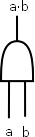
\includegraphics[height=4cm]{images/3-5-andgate.png} &
                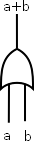
\includegraphics[height=4cm]{images/3-5-orgate.png} &
                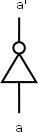
\includegraphics[height=4cm]{images/3-5-notgate.png}
                \\ \\
                \begin{tabular}{ c c | c }
                    $a$ & $b$ & $a \cdot b$ \\ \hline
                    0 & 0 & 0 \\
                    0 & 1 & 0 \\
                    1 & 0 & 0 \\
                    1 & 1 & 1
                \end{tabular}
                &

                \begin{tabular}{ c c | c }
                    $a$ & $b$ & $a + b$ \\ \hline
                    0 & 0 & 0 \\
                    0 & 1 & 1 \\
                    1 & 0 & 1 \\
                    1 & 1 & 1
                \end{tabular}
                &

                \begin{tabular}{ c | c }
                    $a$ & $a'$ \\ \hline
                    0 & 1 \\
                    1 & 0
                \end{tabular}
            \end{tabular}

        \end{center}

            ~\\
            Additionally, we can connect gates together in order to build an expression.
            For example:

        \begin{center}
            \begin{tabular}{c c c}
                $(a+b)'$ &
                $ ab + b' $ &
                $(a+b) \cdot (b' + c)$
                \\
                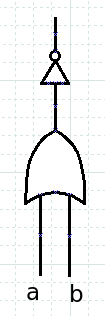
\includegraphics[height=6cm]{images/3-5-gate1.png} &
                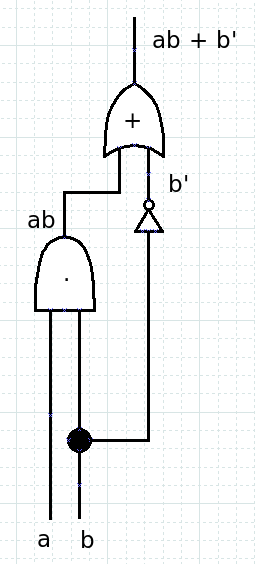
\includegraphics[height=6cm]{images/3-5-gate2.png} &
                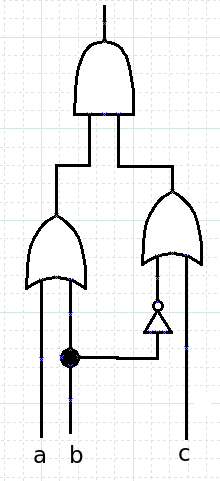
\includegraphics[height=6cm]{images/3-5-gate3.png}
            \end{tabular}
        \end{center}

    \end{intro}

        \newpage

        % - QUESTION --------------------------------------------------%
        \stepcounter{question}
        \begin{questionNOGRADE}{\thequestion}

            Write out the Boolean expression that describes each diagram:


            \begin{center}
                \begin{tabular}{c | c | c}
                    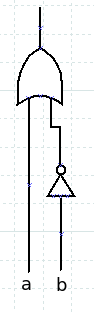
\includegraphics[height=8cm]{images/3-5-gate4.png} &
                    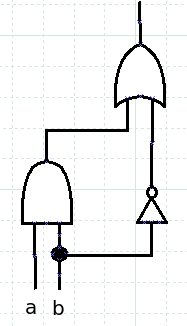
\includegraphics[height=8cm]{images/3-5-gate5.png} &
                    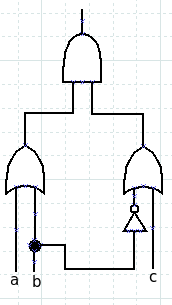
\includegraphics[height=8cm]{images/3-5-gate6.png}
                    \\ & &
                    \\ & &
                    \\ & &
                    \\  \solution{ $a + b'$ }{}
                    &   \solution{ $(a \cdot b) + b'$ }{}
                    &   \solution{ $ (a+b) \cdot (b'+c) $ }{}
                \end{tabular}
            \end{center}


        \end{questionNOGRADE}

        \newpage

        % - QUESTION --------------------------------------------------%
        \stepcounter{question}
        \begin{questionNOGRADE}{\thequestion}

            Draw a circuit diagram for the following Boolean expressions:

            \begin{tabular}{p{4cm} | p{4cm} | p{4cm}}
                a. $a + b'$ &
                b. $a' \cdot b'$ &
                c. $a + (b \cdot c)$
                \\
                FIXME
                \solution{ 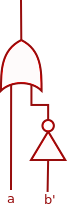
\includegraphics{images/3-5-answer1.png} }{} &
                \solution{ 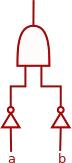
\includegraphics{images/3-5-answer2.png} }{} &
                \solution{ 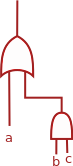
\includegraphics{images/3-5-answer3.png} }{}
            \end{tabular}


        \end{questionNOGRADE}


        \newpage

        \subsection{2-variable Karnaugh Maps}

        \begin{intro}{2x2 Karnaugh Map basics}
            We can use Karnaugh maps to visually represent Boolean expressions
            in order to simplify them. For an expression with two variables,
            our map will be a 2x2 grid like this:

            \begin{center}
                \begin{tabular}{c c c}
                    & $y$ & $y'$ \\ \cline{2-3}
                    $x$     & \multicolumn{1}{|c}{ } & \multicolumn{1}{|c|}{ } \\ \cline{2-3}
                    $x'$    & \multicolumn{1}{|c}{ } & \multicolumn{1}{|c|}{ } \\ \cline{2-3}
                \end{tabular}
            \end{center}

            If you have one product in your equation, you check off the cell where the terms intersect:

            $xy$:
                \begin{tabular}{c c c}
                    & $y$ & $y'$ \\ \cline{2-3}
                    $x$     & \multicolumn{1}{|c}{\checkmark } & \multicolumn{1}{|c|}{ } \\ \cline{2-3}
                    $x'$    & \multicolumn{1}{|c}{ } & \multicolumn{1}{|c|}{ } \\ \cline{2-3}
                \end{tabular}
            \tab $x'y$:
                \begin{tabular}{c c c}
                    & $y$ & $y'$ \\ \cline{2-3}
                    $x$     & \multicolumn{1}{|c}{ } & \multicolumn{1}{|c|}{ } \\ \cline{2-3}
                    $x'$    & \multicolumn{1}{|c}{ \checkmark } & \multicolumn{1}{|c|}{ } \\ \cline{2-3}
                \end{tabular}
            \tab $xy'$:
                \begin{tabular}{c c c}
                    & $y$ & $y'$ \\ \cline{2-3}
                    $x$     & \multicolumn{1}{|c}{ } & \multicolumn{1}{|c|}{ \checkmark } \\ \cline{2-3}
                    $x'$    & \multicolumn{1}{|c}{  } & \multicolumn{1}{|c|}{ } \\ \cline{2-3}
                \end{tabular}

            ~\\~\\
            Each product translates to a cell being \checkmark 'd. When there are multiple products,
            they're added with +:

            $xy + x'y$:
                \begin{tabular}{c c c}
                    & $y$ & $y'$ \\ \cline{2-3}
                    $x$     & \multicolumn{1}{|c}{ \checkmark } & \multicolumn{1}{|c|}{ } \\ \cline{2-3}
                    $x'$    & \multicolumn{1}{|c}{ \checkmark } & \multicolumn{1}{|c|}{ } \\ \cline{2-3}
                \end{tabular}
            \tab $xy + xy' + x'y'$:
                \begin{tabular}{c c c}
                    & $y$ & $y'$ \\ \cline{2-3}
                    $x$     & \multicolumn{1}{|c}{ \checkmark } & \multicolumn{1}{|c|}{ \checkmark } \\ \cline{2-3}
                    $x'$    & \multicolumn{1}{|c}{  } & \multicolumn{1}{|c|}{ \checkmark } \\ \cline{2-3}
                \end{tabular}

        \end{intro}


        % - QUESTION --------------------------------------------------%
        \stepcounter{question}
        \begin{questionNOGRADE}{\thequestion}

            Check off all appropriate term cells for the following maps.

            \begin{center}
                \begin{tabular}{p{4cm} p{4cm} p{4cm}}
                    a. $xy$ & b. $xy + xy'$ & c. $xy + x'y' + x'y$
                    \\
                    \begin{tabular}{c c c}
                        & $y$ & $y'$ \\ \cline{2-3}
                        $x$     & \multicolumn{1}{|c}{ \solution{\checkmark}{} }
                                & \multicolumn{1}{|c|}{ } \\ \cline{2-3}
                        $x'$    & \multicolumn{1}{|c}{ }
                                & \multicolumn{1}{|c|}{ } \\ \cline{2-3}
                    \end{tabular}
                    &
                    \begin{tabular}{c c c}
                        & $y$ & $y'$ \\ \cline{2-3}
                        $x$     & \multicolumn{1}{|c}{ \solution{\checkmark}{} }
                                & \multicolumn{1}{|c|}{ \solution{\checkmark}{} } \\ \cline{2-3}
                        $x'$    & \multicolumn{1}{|c}{ }
                                & \multicolumn{1}{|c|}{ } \\ \cline{2-3}
                    \end{tabular}
                    &
                    \begin{tabular}{c c c}
                        & $y$ & $y'$ \\ \cline{2-3}
                        $x$     & \multicolumn{1}{|c}{ \solution{\checkmark}{} }
                                & \multicolumn{1}{|c|}{ } \\ \cline{2-3}
                        $x'$    & \multicolumn{1}{|c}{ \solution{\checkmark}{} }
                                & \multicolumn{1}{|c|}{ \solution{\checkmark}{} } \\ \cline{2-3}
                    \end{tabular}

                \end{tabular}
            \end{center}

        \end{questionNOGRADE}

    \newpage


        \begin{intro}{One region}

            After writing out all of the products, any \underline{adjacent} cells can be grouped off
            within a rectangular region. For a $2x2$ grid, our grouping rectangles can be $1x1$ (no simplification), $2x1$, $1x2$, or $2x2$.

            \begin{center}
                $xy + x'y$:
                \begin{tabular}{c c c}
                    & $y$ & $y'$ \\ \cline{2-3}
                    $x$     & \multicolumn{1}{|c}{ \cellcolor{red!50}\checkmark } & \multicolumn{1}{|c|}{ } \\ \cline{2-3}
                    $x'$    & \multicolumn{1}{|c}{ \cellcolor{red!50}\checkmark } & \multicolumn{1}{|c|}{ } \\ \cline{2-3}
                \end{tabular}
            \end{center}

            When you have a rectangular region, you can remove one of the variables. Whichever
            variable has both the \textbf{normal} and \textbf{prime} version can be removed.

            \begin{center}
                $xy + x'y$:
                \begin{tabular}{c c c}
                    & $y$ & $y'$ \\ \cline{2-3}
                    $x$     & \multicolumn{1}{|c}{ \cellcolor{red!50}\checkmark } & \multicolumn{1}{|c|}{ } \\ \cline{2-3}
                    $x'$    & \multicolumn{1}{|c}{ \cellcolor{red!50}\checkmark } & \multicolumn{1}{|c|}{ } \\ \cline{2-3}
                \end{tabular}

                ~\\ $xy + x'y$ $\Rightarrow$ Remove the $x$ variable, change to $y$
            \end{center}
        \end{intro}


        % - QUESTION --------------------------------------------------%
        \stepcounter{question}
        \begin{questionNOGRADE}{\thequestion}

            Fill out the map, outline adjacent regions, and eliminate one variable.

            \begin{center}
                \begin{tabular}{p{4cm} p{4cm} p{4cm}}
                    a. $xy + xy'$
                    & b. $x'y + xy$
                    & c. $x'y' + x'y$
                    \\
                    \begin{tabular}{c c c}
                        & $y$ & $y'$ \\ \cline{2-3}
                        $x$     & \multicolumn{1}{|c}{ \solution{\cellcolor{red!25}\checkmark}{} }
                                & \multicolumn{1}{|c|}{ \solution{\cellcolor{red!25}\checkmark}{} } \\ \cline{2-3}
                        $x'$    & \multicolumn{1}{|c}{ }
                                & \multicolumn{1}{|c|}{ } \\ \cline{2-3}
                    \end{tabular}
                    &
                    \begin{tabular}{c c c}
                        & $y$ & $y'$ \\ \cline{2-3}
                        $x$     & \multicolumn{1}{|c}{ \solution{\cellcolor{red!25}\checkmark}{} }
                                & \multicolumn{1}{|c|}{ } \\ \cline{2-3}
                        $x'$    & \multicolumn{1}{|c}{ \solution{\cellcolor{red!25}\checkmark}{} }
                                & \multicolumn{1}{|c|}{ } \\ \cline{2-3}
                    \end{tabular}
                    &
                    \begin{tabular}{c c c}
                        & $y$ & $y'$ \\ \cline{2-3}
                        $x$     & \multicolumn{1}{|c}{ }
                                & \multicolumn{1}{|c|}{  } \\ \cline{2-3}
                        $x'$    & \multicolumn{1}{|c}{ \solution{\cellcolor{red!25}\checkmark}{} }
                                & \multicolumn{1}{|c|}{ \solution{\cellcolor{red!25}\checkmark}{} } \\ \cline{2-3}
                    \end{tabular}
                    \\
                    \\
                    \solution{= $x$}{}
                    & \solution{= $y$}{}
                    & \solution{= $x'$}{}

                \end{tabular}
            \end{center}

        \end{questionNOGRADE}

        \newpage

        \begin{intro}{Multiple regions}
            If you can highlight multiple regions, you will end up with that amount of terms,
            combined by Boolean addition +.

            \paragraph{Example:} We have the expression $xy + xy' + x'y$, our map looks like this:

                \begin{center}
                    \begin{tabular}{c c c}
                        & $y$ & $y'$ \\ \cline{2-3}
                        $x$     & \multicolumn{1}{|c }{ \checkmark }
                                & \multicolumn{1}{|c|}{ \checkmark } \\ \cline{2-3}
                        $x'$    & \multicolumn{1}{|c }{ \checkmark }
                                & \multicolumn{1}{|c|}{  } \\ \cline{2-3}
                    \end{tabular}
                \end{center}

                We will have two regions...

                This
                    \begin{tabular}{c c c}
                        & $y$ & $y'$ \\ \cline{2-3}
                        $x$     & \multicolumn{1}{|c }{ \cellcolor{red!50}\checkmark }
                                & \multicolumn{1}{|c|}{ \cellcolor{red!50}\checkmark } \\ \cline{2-3}
                        $x'$    & \multicolumn{1}{|c }{ \checkmark }
                                & \multicolumn{1}{|c|}{  } \\ \cline{2-3}
                    \end{tabular}
                \tab and this
                    \begin{tabular}{c c c}
                        & $y$ & $y'$ \\ \cline{2-3}
                        $x$     & \multicolumn{1}{|c }{ \cellcolor{red!50}\checkmark }
                                & \multicolumn{1}{|c|}{ \checkmark } \\ \cline{2-3}
                        $x'$    & \multicolumn{1}{|c }{ \cellcolor{red!50}\checkmark }
                                & \multicolumn{1}{|c|}{  } \\ \cline{2-3}
                    \end{tabular}

                ~\\~\\
                So our two terms will be $x$ and $y$. Therefore, we can simplify
                \begin{center}
                    $xy + xy' + x'y$

                    to

                    $x + y$
                \end{center}
        \end{intro}

        % - QUESTION --------------------------------------------------%
        \stepcounter{question}
        \begin{questionNOGRADE}{\thequestion}

            Use Karnaugh maps to simplify the following expressions.

            ~\\
            \begin{tabular}{p{6cm} p{6cm}}
                a. $xy' + x'y'$ & b. $xy + x'y + x'y'$ \\
                    \begin{tabular}{c c c}
                        & $y$ & $y'$ \\ \cline{2-3}
                        $x$     & \multicolumn{1}{|c }{  }
                                & \multicolumn{1}{|c|}{ \solution{ \cellcolor{red!25}\checkmark }{} } \\ \cline{2-3}
                        $x'$    & \multicolumn{1}{|c }{  }
                                & \multicolumn{1}{|c|}{ \solution{ \cellcolor{red!25}\checkmark }{} } \\ \cline{2-3}
                    \end{tabular}
                    &

                    \begin{tabular}{c c c}
                        & $y$ & $y'$ \\ \cline{2-3}
                        $x$     & \multicolumn{1}{|c }{ \solution{ \cellcolor{red!25}\checkmark }{} }
                                & \multicolumn{1}{|c|}{  } \\ \cline{2-3}
                        $x'$    & \multicolumn{1}{|c }{ \solution{ \cellcolor{red!25}\checkmark }{} }
                                & \multicolumn{1}{|c|}{ \solution{ \cellcolor{red!25}\checkmark }{} } \\ \cline{2-3}
                    \end{tabular}

                    \\ \\
                    \solution{= $y'$ }{} &
                    \solution{= $x' + y$ }{}

            \end{tabular}
        \end{questionNOGRADE}



        \newpage
        \subsection{3-variable Karnaugh Maps}

        \begin{intro}{\ }
            Once we have three variables, we will have to change our map.
            It will become a $2x4$ map, where each column represents \textbf{two variables}.
            \begin{center}
                \begin{tabular}{c c c c c}
                    & $yz$ & $yz'$ & $y'z'$ & $y'z$ \\ \cline{2-5}
                    $x$     & \multicolumn{1}{|c }{  }
                            & \multicolumn{1}{|c }{  }
                            & \multicolumn{1}{|c }{  }
                            & \multicolumn{1}{|c|}{  } \\ \cline{2-5}
                    $x'$    & \multicolumn{1}{|c }{  }
                            & \multicolumn{1}{|c }{  }
                            & \multicolumn{1}{|c }{  }
                            & \multicolumn{1}{|c|}{  } \\ \cline{2-5}
                \end{tabular}
            \end{center}

            Note that for each column, the difference between any two columns
            can be only \textbf{one}... in other words, you can go from $yz$ to $y'z$ or $yz'$, but
            you CANNOT go from $yz$ to $y'z'$.

            We can then follow the same approach to mark off cells that correspond to products of terms:

            \begin{center}
                \begin{tabular}{c c c c c}
                    & $yz$ & $yz'$ & $y'z'$ & $y'z$ \\ \cline{2-5}
                    $x$     & \multicolumn{1}{|c }{ \checkmark }
                            & \multicolumn{1}{|c }{  }
                            & \multicolumn{1}{|c }{  }
                            & \multicolumn{1}{|c|}{  } \\ \cline{2-5}
                    $x'$    & \multicolumn{1}{|c }{ \checkmark }
                            & \multicolumn{1}{|c }{  }
                            & \multicolumn{1}{|c }{  }
                            & \multicolumn{1}{|c|}{  } \\ \cline{2-5}
                \end{tabular}
                ~\\~\\
                $xyz + x'yz$
            \end{center}

            We can also highlight regions in order to simplify the expression.
            For a $2x4$ Karnaugh map, our regions can be...:
            $1x1$   (no simplification), $2x1$, $1x2$, or $2x2$.

            \paragraph{Example:} Simplify $x'yz + x'y'z + xyz' + xy'z'$
            \begin{center}
                \begin{tabular}{c c c c c}
                    & $yz$ & $yz'$ & $y'z'$ & $y'z$ \\ \cline{2-5}
                    $x$     & \multicolumn{1}{|c }{  }
                            & \multicolumn{1}{|c }{ \checkmark }
                            & \multicolumn{1}{|c }{ \checkmark }
                            & \multicolumn{1}{|c|}{  } \\ \cline{2-5}
                    $x'$    & \multicolumn{1}{|c }{ \checkmark }
                            & \multicolumn{1}{|c }{  }
                            & \multicolumn{1}{|c }{  }
                            & \multicolumn{1}{|c|}{ \checkmark } \\ \cline{2-5}
                \end{tabular}
            \end{center}

            We can also \textit{wrap around} horizontally; the checkmarks at
            $x'yz$ and $x'y'z$ can be counted as one region.
            \begin{center}
                \begin{tabular}{c c c c c}
                    & $yz$ & $yz'$ & $y'z'$ & $y'z$ \\ \cline{2-5}
                    $x$     & \multicolumn{1}{|c }{  }
                            & \multicolumn{1}{|c }{ \cellcolor{red!25}\checkmark }
                            & \multicolumn{1}{|c }{ \cellcolor{red!25}\checkmark }
                            & \multicolumn{1}{|c|}{  } \\ \cline{2-5}
                    $x'$    & \multicolumn{1}{|c }{ \cellcolor{green!25}\checkmark }
                            & \multicolumn{1}{|c }{  }
                            & \multicolumn{1}{|c }{  }
                            & \multicolumn{1}{|c|}{ \cellcolor{green!25}\checkmark } \\ \cline{2-5}
                \end{tabular}
            \end{center}

            We have two regions, so we can simplify it into two terms.
            Any variables in a region that have both the normal and prime versions
            stay, any variable that is the same for all cells in the region are removed.

            \begin{center}
                $x'yz + x'y'z + xyz' + xy'z' \tab \Rightarrow \tab xz' + x'z$
            \end{center}
        \end{intro}

        \begin{intro}{\ }
            \textbf{More rules...}

            \paragraph{Choosing regions:}
            Sometimes you can come up with multiple regions in your map.
            What is the best way to make your regions? In order to get
            the simplest expression, choose the \textit{smallest amount of rectangles},
            and such that \textit{each rectangle is as large as possible.}

            \paragraph{1x1 regions} You can choose a 1x1 region if
            doing so allows you to have largest-possible-regions for other terms.

        \end{intro}

        % - QUESTION --------------------------------------------------%
        \stepcounter{question}
        \begin{questionNOGRADE}{\thequestion}
            Simplify the following equations with a Karnaugh map.

            \begin{enumerate}
                \item[a.]   $xyz + xyz' + xy'z' + xy'z$

                \begin{tabular}{c c c c c}
                    & $yz$ & $yz'$ & $y'z'$ & $y'z$ \\ \cline{2-5}
                    $x$     & \multicolumn{1}{|c }{ \solution{\checkmark}{} }
                            & \multicolumn{1}{|c }{ \solution{\checkmark}{} }
                            & \multicolumn{1}{|c }{ \solution{\checkmark}{} }
                            & \multicolumn{1}{|c|}{ \solution{\checkmark}{} } \\ \cline{2-5}
                    $x'$    & \multicolumn{1}{|c }{  }
                            & \multicolumn{1}{|c }{  }
                            & \multicolumn{1}{|c }{  }
                            & \multicolumn{1}{|c|}{  } \\ \cline{2-5}
                \end{tabular}

                \solution{ ~\\ = $x$}{ ~\\~\\ }

                \item[b.]   $xyz + xyz' + x'yz + x'yz'$

                \begin{tabular}{c c c c c}
                    & $yz$ & $yz'$ & $y'z'$ & $y'z$ \\ \cline{2-5}
                    $x$     & \multicolumn{1}{|c }{ \solution{\checkmark}{} }
                            & \multicolumn{1}{|c }{ \solution{\checkmark}{} }
                            & \multicolumn{1}{|c }{  }
                            & \multicolumn{1}{|c|}{  } \\ \cline{2-5}
                    $x'$    & \multicolumn{1}{|c }{ \solution{\checkmark}{} }
                            & \multicolumn{1}{|c }{ \solution{\checkmark}{} }
                            & \multicolumn{1}{|c }{  }
                            & \multicolumn{1}{|c|}{  } \\ \cline{2-5}
                \end{tabular}

                \solution{ ~\\ = $y$}{ ~\\~\\ }

                \item[c.]   $xyz + xyz' + x'y'z' + x'y'z$

                \begin{tabular}{c c c c c}
                    & $yz$ & $yz'$ & $y'z'$ & $y'z$ \\ \cline{2-5}
                    $x$     & \multicolumn{1}{|c }{ \solution{\checkmark}{} }
                            & \multicolumn{1}{|c }{ \solution{\checkmark}{} }
                            & \multicolumn{1}{|c }{  }
                            & \multicolumn{1}{|c|}{  } \\ \cline{2-5}
                    $x'$    & \multicolumn{1}{|c }{  }
                            & \multicolumn{1}{|c }{  }
                            & \multicolumn{1}{|c }{ \solution{\checkmark}{} }
                            & \multicolumn{1}{|c|}{ \solution{\checkmark}{} } \\ \cline{2-5}
                \end{tabular}

                \solution{ ~\\ = $xy + x'y'$}{ ~\\~\\ }

                \item[d.]   $x'y'z' + xyz + xyz' + xy'z' + xy'z$

                \begin{tabular}{c c c c c}
                    & $yz$ & $yz'$ & $y'z'$ & $y'z$ \\ \cline{2-5}
                    $x$     & \multicolumn{1}{|c }{ \solution{\checkmark}{} }
                            & \multicolumn{1}{|c }{ \solution{\checkmark}{} }
                            & \multicolumn{1}{|c }{ \solution{\checkmark}{} }
                            & \multicolumn{1}{|c|}{ \solution{\checkmark}{} } \\ \cline{2-5}
                    $x'$    & \multicolumn{1}{|c }{  }
                            & \multicolumn{1}{|c }{  }
                            & \multicolumn{1}{|c }{ \solution{\checkmark}{} }
                            & \multicolumn{1}{|c|}{  } \\ \cline{2-5}
                \end{tabular}

                \solution{ ~\\ = $x + y'z'$}{}
            \end{enumerate}
        \end{questionNOGRADE}






\end{document}








